\documentclass{beamer}
\usepackage{amsmath,amsthm,ifthen}
\usepackage{uofmtheme}
\title{Spring Introduce Extension}
\author{John Chilton}

\begin{document}
\frame{\titlepage}

\section{Introduction}
\subsection{Outline}
\frame{
The Spring extension builds on top of the Interfaces extension providing all of the same benefits for the service developer and the user of the service.
~\\
~\\
The Spring extension provides two additional features for the service developer. 
\begin{itemize}
 \item Spring beans may be annotated as implementing interfaces for a service from inside of a Spring configuration file.
 \item Spring beans may be configured to act as proxies for getting and setting WSRF resource properties.
\end{itemize}
}

\subsection{Example Service}

\frame{
To demonstrate the Spring extension we will recreate the \texttt{CalculatorService} service, but this time we will place the operations in a service context. This will make it easier to demonstrate working with resource properties. Both extensions can be used however to manage operations on a main service and/or its service contexts.
}


\frame{
\begin{columns}
\column{3cm}
Recreate the CalculatorService, this time with the SpringExtension.
\column{7cm}
\begin{center}
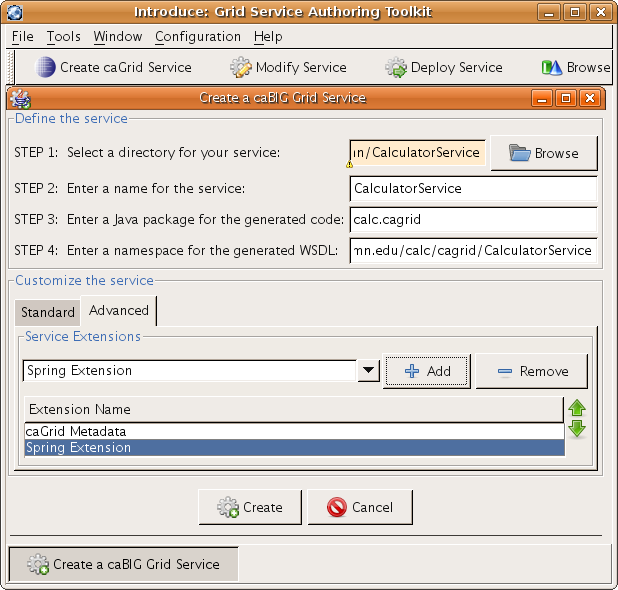
\includegraphics[scale=.30]{images/springCreate.png}  
\end{center}
\end{columns}
}

\frame{
\begin{columns}
\column{7cm}
\begin{center}
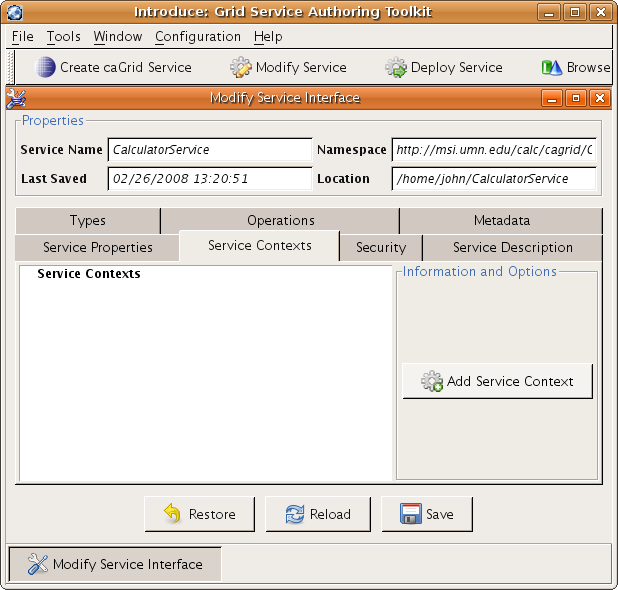
\includegraphics[scale=.30]{images/springContext.png}  
\end{center}
\column{3cm}
Select the ``Service Contexts'' tab, then click the ``Add Service Context'' button.
\end{columns}
}

\frame{
\begin{columns}
\column{3cm}
Click the ``Done'' button.
\column{7cm}
\begin{center}
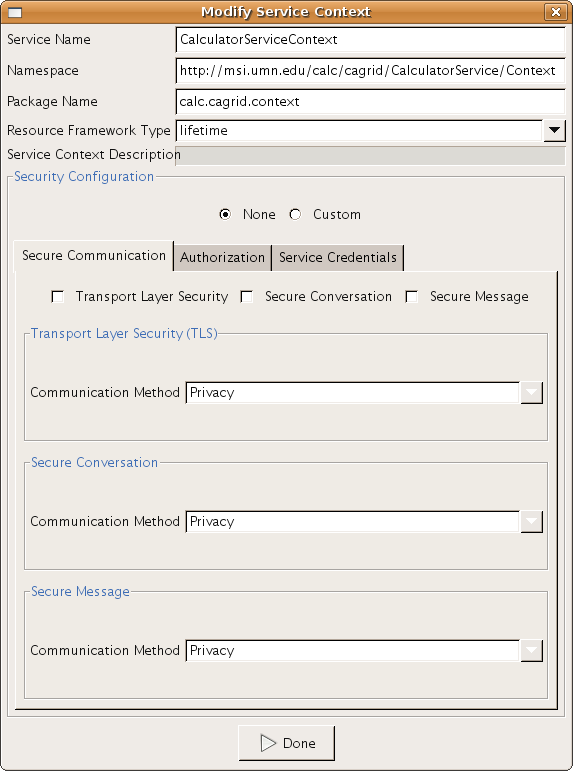
\includegraphics[scale=.25]{images/springContextCreate.png}  
\end{center}
\end{columns}
}

\frame{
\begin{columns}
\column{7cm}
\begin{center}
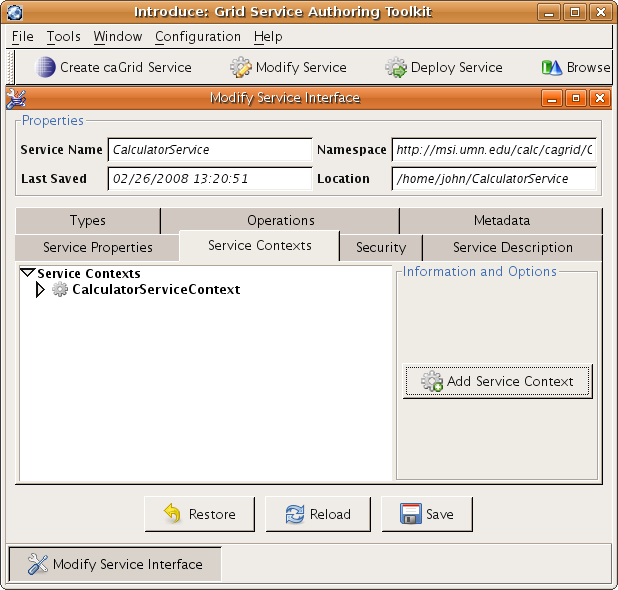
\includegraphics[scale=.30]{images/springContextCreated.png}  
\end{center}
\column{3cm}
The service is now setup.
\end{columns}
} 
\section{\ttfamily implements-for-service}
\subsection{\ttfamily applicationContext.xml}
\frame{
\frametitle{applicationContext.xml (1 / 3)}
The Spring extension creates the outline of a Spring configuration file and places it in the \texttt{etc} directory.
\begin{block}{\ttfamily etc/applicationContext.xml}\ttfamily
<?xml version="1.0" encoding="UTF-8"?> \\
<beans xmlns="http://www.springframework.org/...." \\
~~xmlns:xsi="http://www.w3.org/..." \\
~~xmlns:spring="http://msi.umn.edu/..." \\
~~xmlns:interfaces="http://msi.umn.edu/..." \\
~~xsi:schemaLocation="...">\\ 
~\\
~~<!-- Define beans and caGrid mappings here --> \\
</beans>
\end{block}
}

\frame{
\frametitle{applicationContext.xml (2 / 3)}
Add the following lines to this file to create a calculator bean and configure it to implement \texttt{Adder} and \texttt{Subtracter} for the \texttt{CalculatorServiceContext} service.
\begin{block}{\ttfamily etc/applicationContext.xml}\ttfamily
<beans ...>\\ 
~~\color{maroon}<bean id="theCalculator" class="calc.Calculator" /> \\
~~<spring:implements-for-service \\
~~~~~~~~~~service="CalculatorServiceContext" \\
~~~~~~~~~~implementer="theCalculator"> \\
~~~~<interfaces:interface name="calc.Adder" /> \\
~~~~<interfaces:interface name="calc.Subtracter" /> \\
~~</spring:implements-for-service>\color{black}\\
</beans>
\end{block}
}

\frame{
\frametitle{applicationContext.xml (3 / 3)}
\begin{block}{Compile Time Versus Runtime}
\texttt{implements-for-service} elements are translated into service operations when Introduce saves. If any part of an \texttt{implements-for-service} element is modified the service should be resaved. If only bean definitions are modified there is no need to resave. 
\end{block}
\begin{block}{Importing Other Spring Files}
The implementer bean definition may come from an imported Spring file, but all of the actual \texttt{implements-for-service} elements must be defined directly in the \texttt{applicationContext.xml} file.
\end{block}
}

\subsection{Demonstration}
\frame{
\begin{columns}
\column{3cm}
After copying the appropriate jar and saving
\column{7cm}
\begin{center}
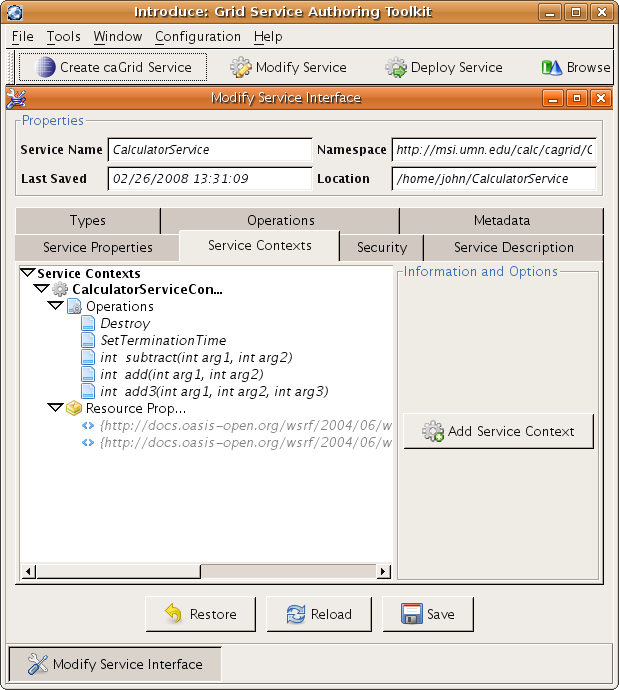
\includegraphics[scale=.30]{images/springSave1.png}  
\end{center}
\end{columns}
}

\section{\ttfamily resource-property}

\frame{
To demonstrate the Spring integration with resource properties we will add a resource property to the service context. We will create a string resource property that will keep track of the last operation called.
}

\frame{
\begin{columns}
\column{3cm}
Select ``Resource Properties'', then click the ``Modifiy Resources'' button.
\column{7cm}
\begin{center}
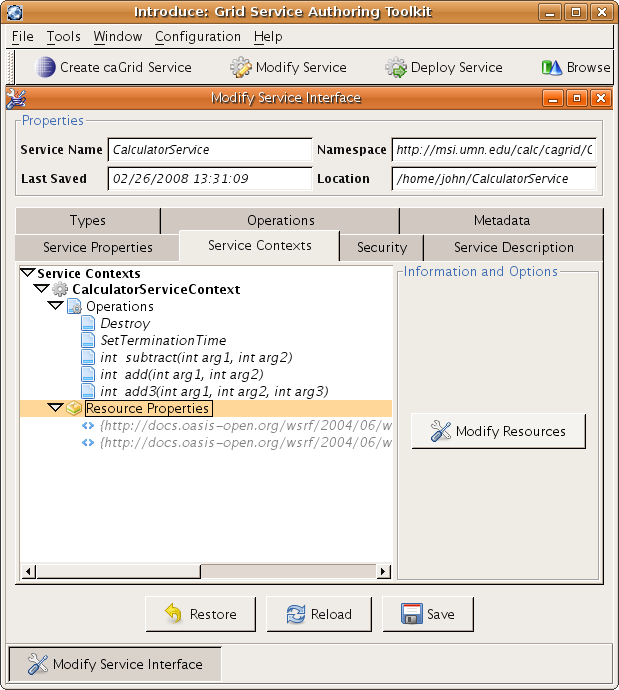
\includegraphics[scale=.30]{images/springModifyResources.png}  
\end{center}
\end{columns}
}

\frame{
\begin{center}
Add a string resource property.
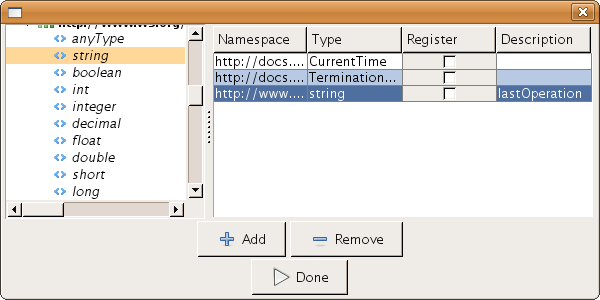
\includegraphics[scale=.50]{images/springResourceProperty.png}  
\end{center}
}

\frame{
\begin{columns}
\column{7cm}
\begin{center}
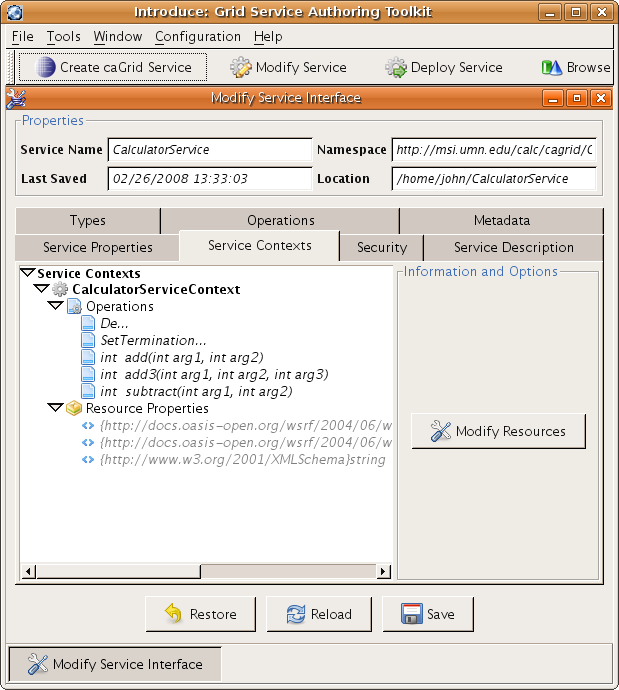
\includegraphics[scale=.30]{images/springWithResourceProperty.png}  
\end{center}
\column{3cm}
After saving, you should see the new resource property.
\end{columns}
}


\frame{
\begin{block}{\ttfamily Calculator.java}\ttfamily
package calc;\\
public class Calculator implements Adder,Subtracter\{\\
~~private Tracker tracker;\\
~ \\
~~public void setTracker(Tracker tracker) \{\\
~~~~this.tracker = tracker;\\
~~\}\\
~\\
~~public int add(int x, int y) \{\\
~~~~tracker.setLastOp("Addition");\\
~~~~return x + y;\\
~~\}\\
\}
\end{block}
}

\frame{
\begin{block}{\ttfamily Tracker.java}\ttfamily
package calc; \\
public class Tracker \{ \\
~~public String theLastOperation;\\
~~public void setLastOp(String theLastOperation) \{\\
~~~~this.theLastOperation = theLastOperation; \\
~~\}\\
~~public String getLastOp() \{ \\
~~~~return theLastOperation; \\
~~\} \\
\} \\
\end{block}
}

\frame{
\begin{block}{\ttfamily etc/applicationContext.xml}\ttfamily
~~<bean id="theCalculator" class="calc.Calculator" \color{maroon}> \\
~~~~<property name="tracker">\\
~~~~~~<bean class="calc.Tracker"> \\
~~~~~~~~<spring:resource-property name="string" \\
~~~~~~~~~~get-method="getLastOp" \\
~~~~~~~~~~set-method="setLastOp" /> \\
~~~~~~</bean> \\
~~~~</property> \\
~~</bean>\\
\end{block}
The \texttt{resource-property} elements says to override this beans \texttt{getLastOp} and \texttt{setLastOp} methods to get and set the resource property \texttt{string}.
}


\frame{
% To create the object that is set as \texttt{theCalculator}'s \texttt{Tracker} t
It should be noted that the \texttt{Tracker} class field \texttt{theLastOperation} does not become the resource property. The \texttt{Tracker} class is subclassed at runtime and \texttt{setLastOp} and \texttt{getLastOp} are overridden to access the resource property.
~\\
~\\
As illustratation, this \texttt{Tracker} definition would also work.
\begin{block}{\ttfamily Tracker.java}\ttfamily
package calc; \\
abstract public class Tracker \{ \\
~~abstract public void setLastOp(String lastOp); \\
~~abstract public String getLastOp();  \\
\} \\
\end{block}
}

\frame{
\frametitle{\texttt{resource-property} and Threads}
Like session or request scoped Spring beans, the behavior overridden methods will be tied to the thread they are invoked from. The thread determines what endpoint reference was invoked and hence what resource to access.
~\\
~\\
\begin{block}{Warning}
If these methods are invoked from a thread that doesn't corrsepond to an Axis request or to a service without the specified resource property, a runtime exception will be thrown.
\end{block}
}

\frame{
% TODO: This is an akward slide
\begin{block}{\ttfamily resource-property}
Any number of beans can expose any number of resource properties, and any resource property can be exposed via any number of beans. The \texttt{get-method} or \texttt{set-method} attributes may be excluded, but not both.
\end{block}
}


\end{document}
